% Use xelatex
\documentclass[12pt]{article}
\usepackage[textwidth=4.5in]{geometry}
\usepackage{fontspec}
\usepackage{graphicx}
\pagestyle{empty}

\setmainfont{Bodoni 72 Oldstyle}

\parindent=0pt
\parskip=1.5\baselineskip

\newcommand*\cats{%
	\par
	\qquad
	\includegraphics[height=2\baselineskip]{cat-left}%
	\hfill
	\includegraphics[height=2\baselineskip]{cat-left2}%
	\hfill
	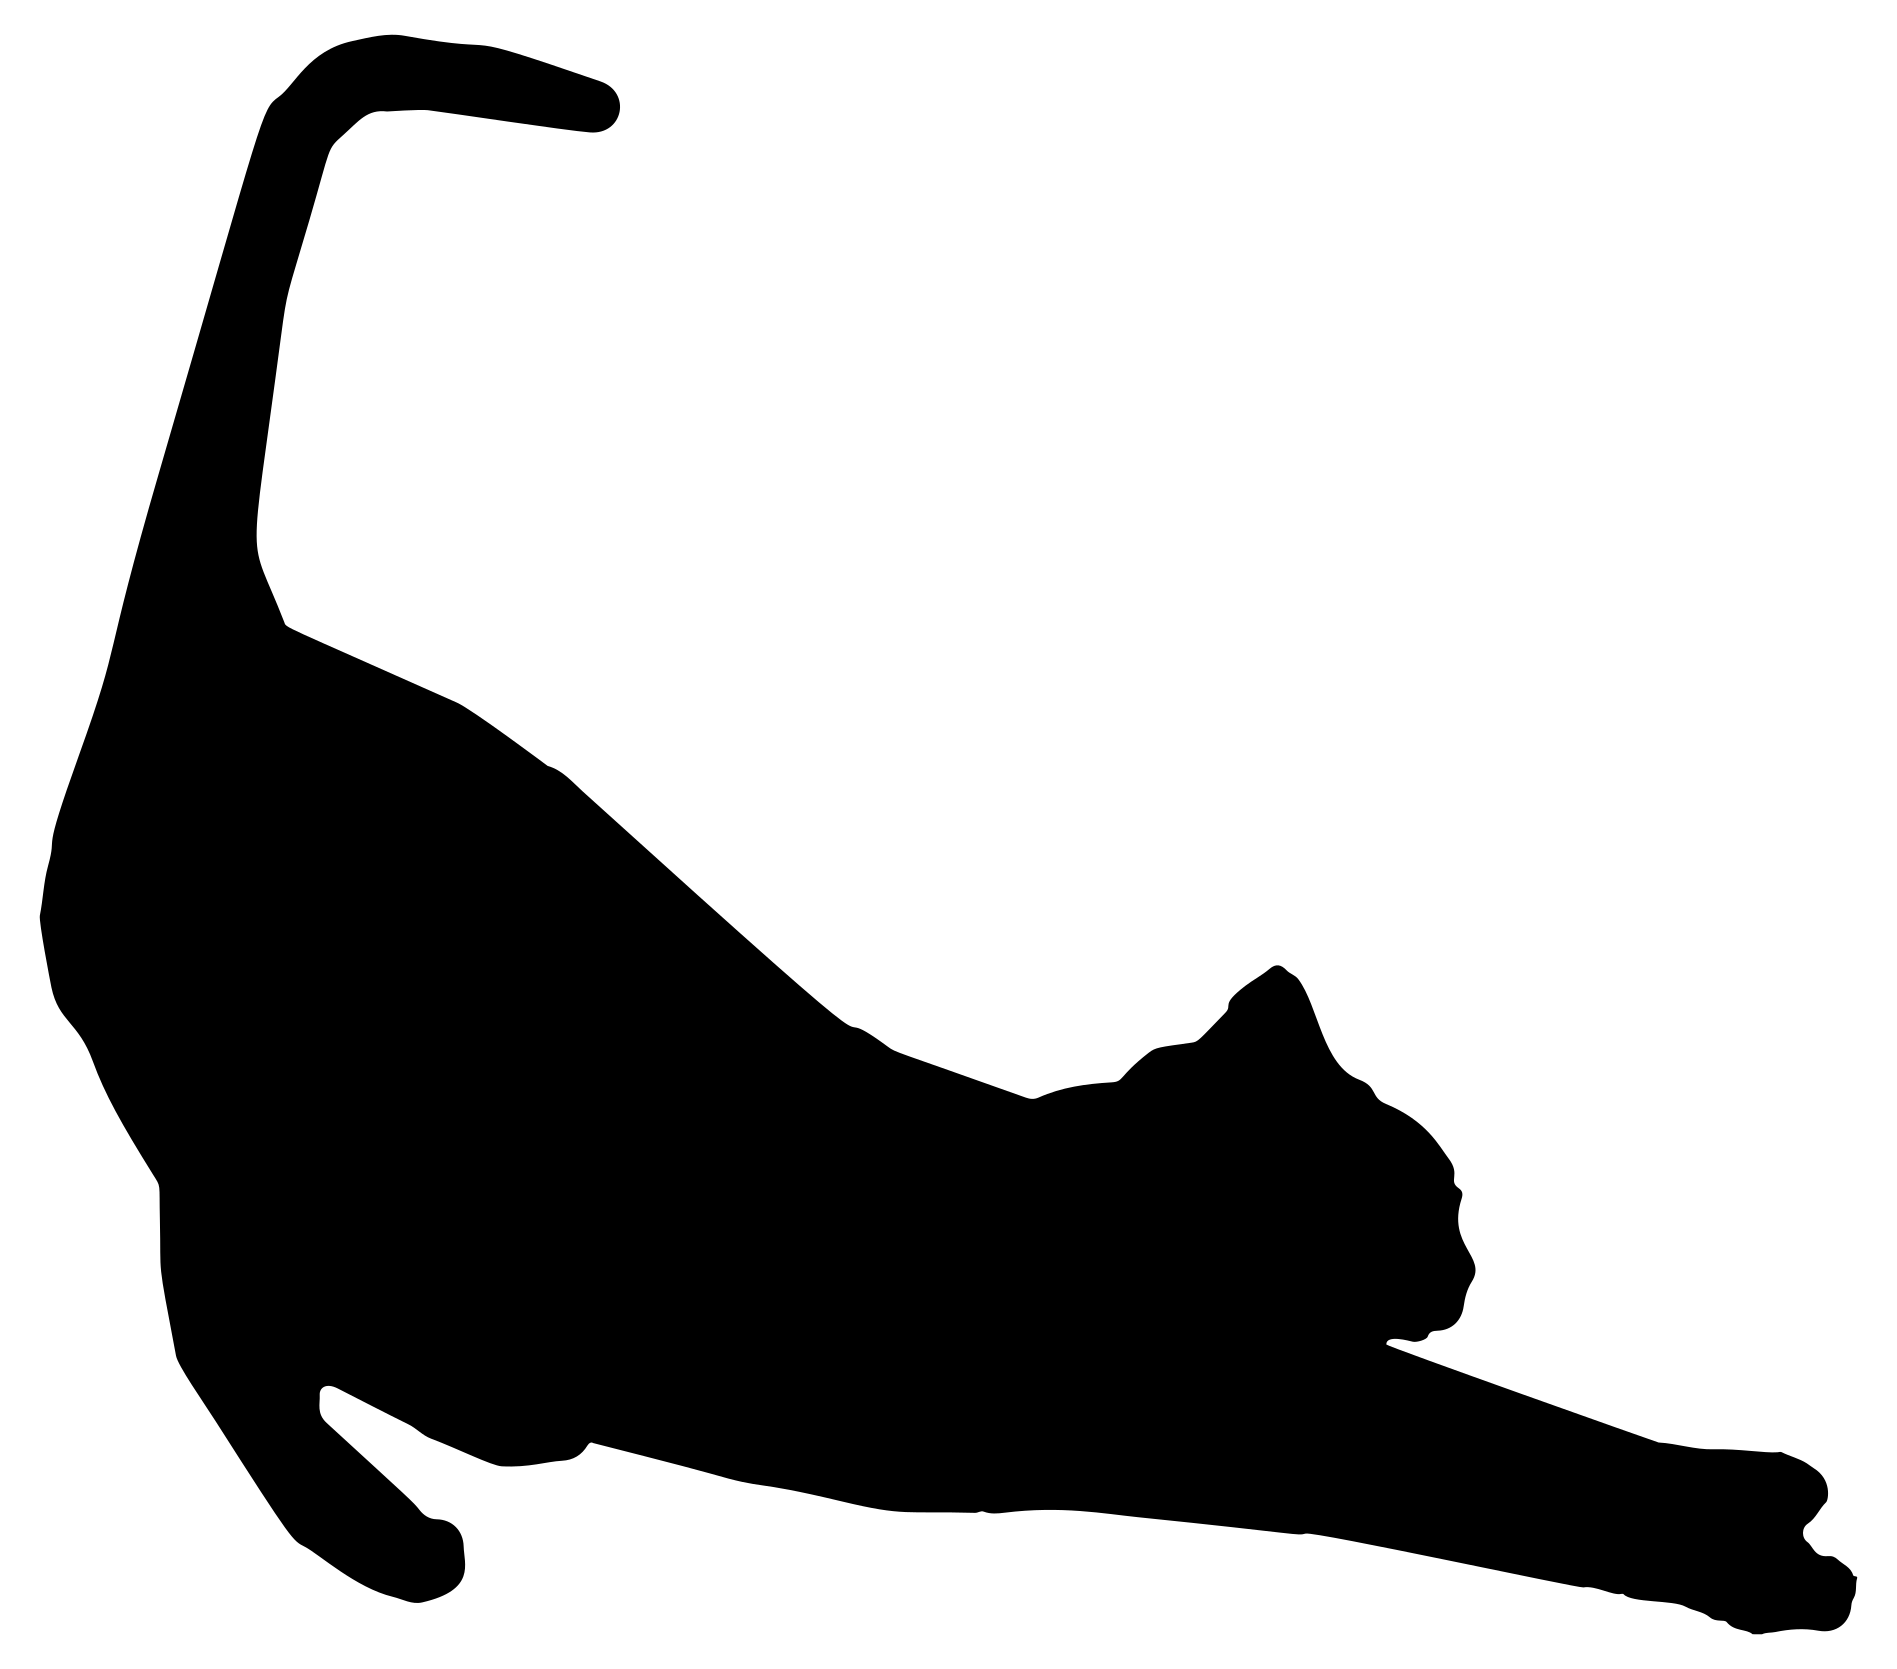
\includegraphics[height=2\baselineskip]{cat-right}%
	\qquad
	\kern0pt
	\par
}
\newcommand*\separator{\hskip.5em\relax$\bullet$\hskip.5em\relax}
\newcommand*\drink[3]{%
	\par
	\textbf{#1}%
	\separator
	\textit{#2}%
	\separator
	#3%
	\par
}

\begin{document}


\cats
\drink{Aviation}{floral, sweet}{gin, creme de violet, lemon}
\drink{Party Cat}{smokey, sparkling}{mezcal, grapefruit, prosecco}
\drink{Lion's Tail}{whiskey christmas}{bourbon, allspice, lime}
\drink{Mai Tai}{sweet, tiki}{rum, almond, lime}
\drink{Tom Collins}{light, refreshing}{old tom gin, lemon, sparking water}
\drink{Malört}{turpentine, fennel}{terroir of chicago}
\drink{Bartender's Choice}{???}{bartender loves gin}
\textbf{An assortment of beers, teas, and sparkling waters}
\cats

\end{document}
